% potato_figures.tex
% Paper figures, drop-in for upload.
%
% Required preamble:
%   \usepackage{graphicx}
%   \usepackage[font=small,labelfont=bf]{caption}
%
% Three figures shipped:
%   FIG 1.  exhibit1_europe.png       --- Europe hex-bin maps
%   FIG 2.  exhibit2_france.png       --- France PROVINC bubble maps
%   FIG 3.  exhibit3_binscatter.png   --- Headline regression binscatter
%                                         (NUTS-2 + France)
% All three .png files should be in the same directory as the main .tex,
% or adjust the \includegraphics path.

% =============================================================
%  FIGURE 1.  Europe: potato suitability vs urban-size dispersion.
% =============================================================

\begin{figure}[!htbp]\centering
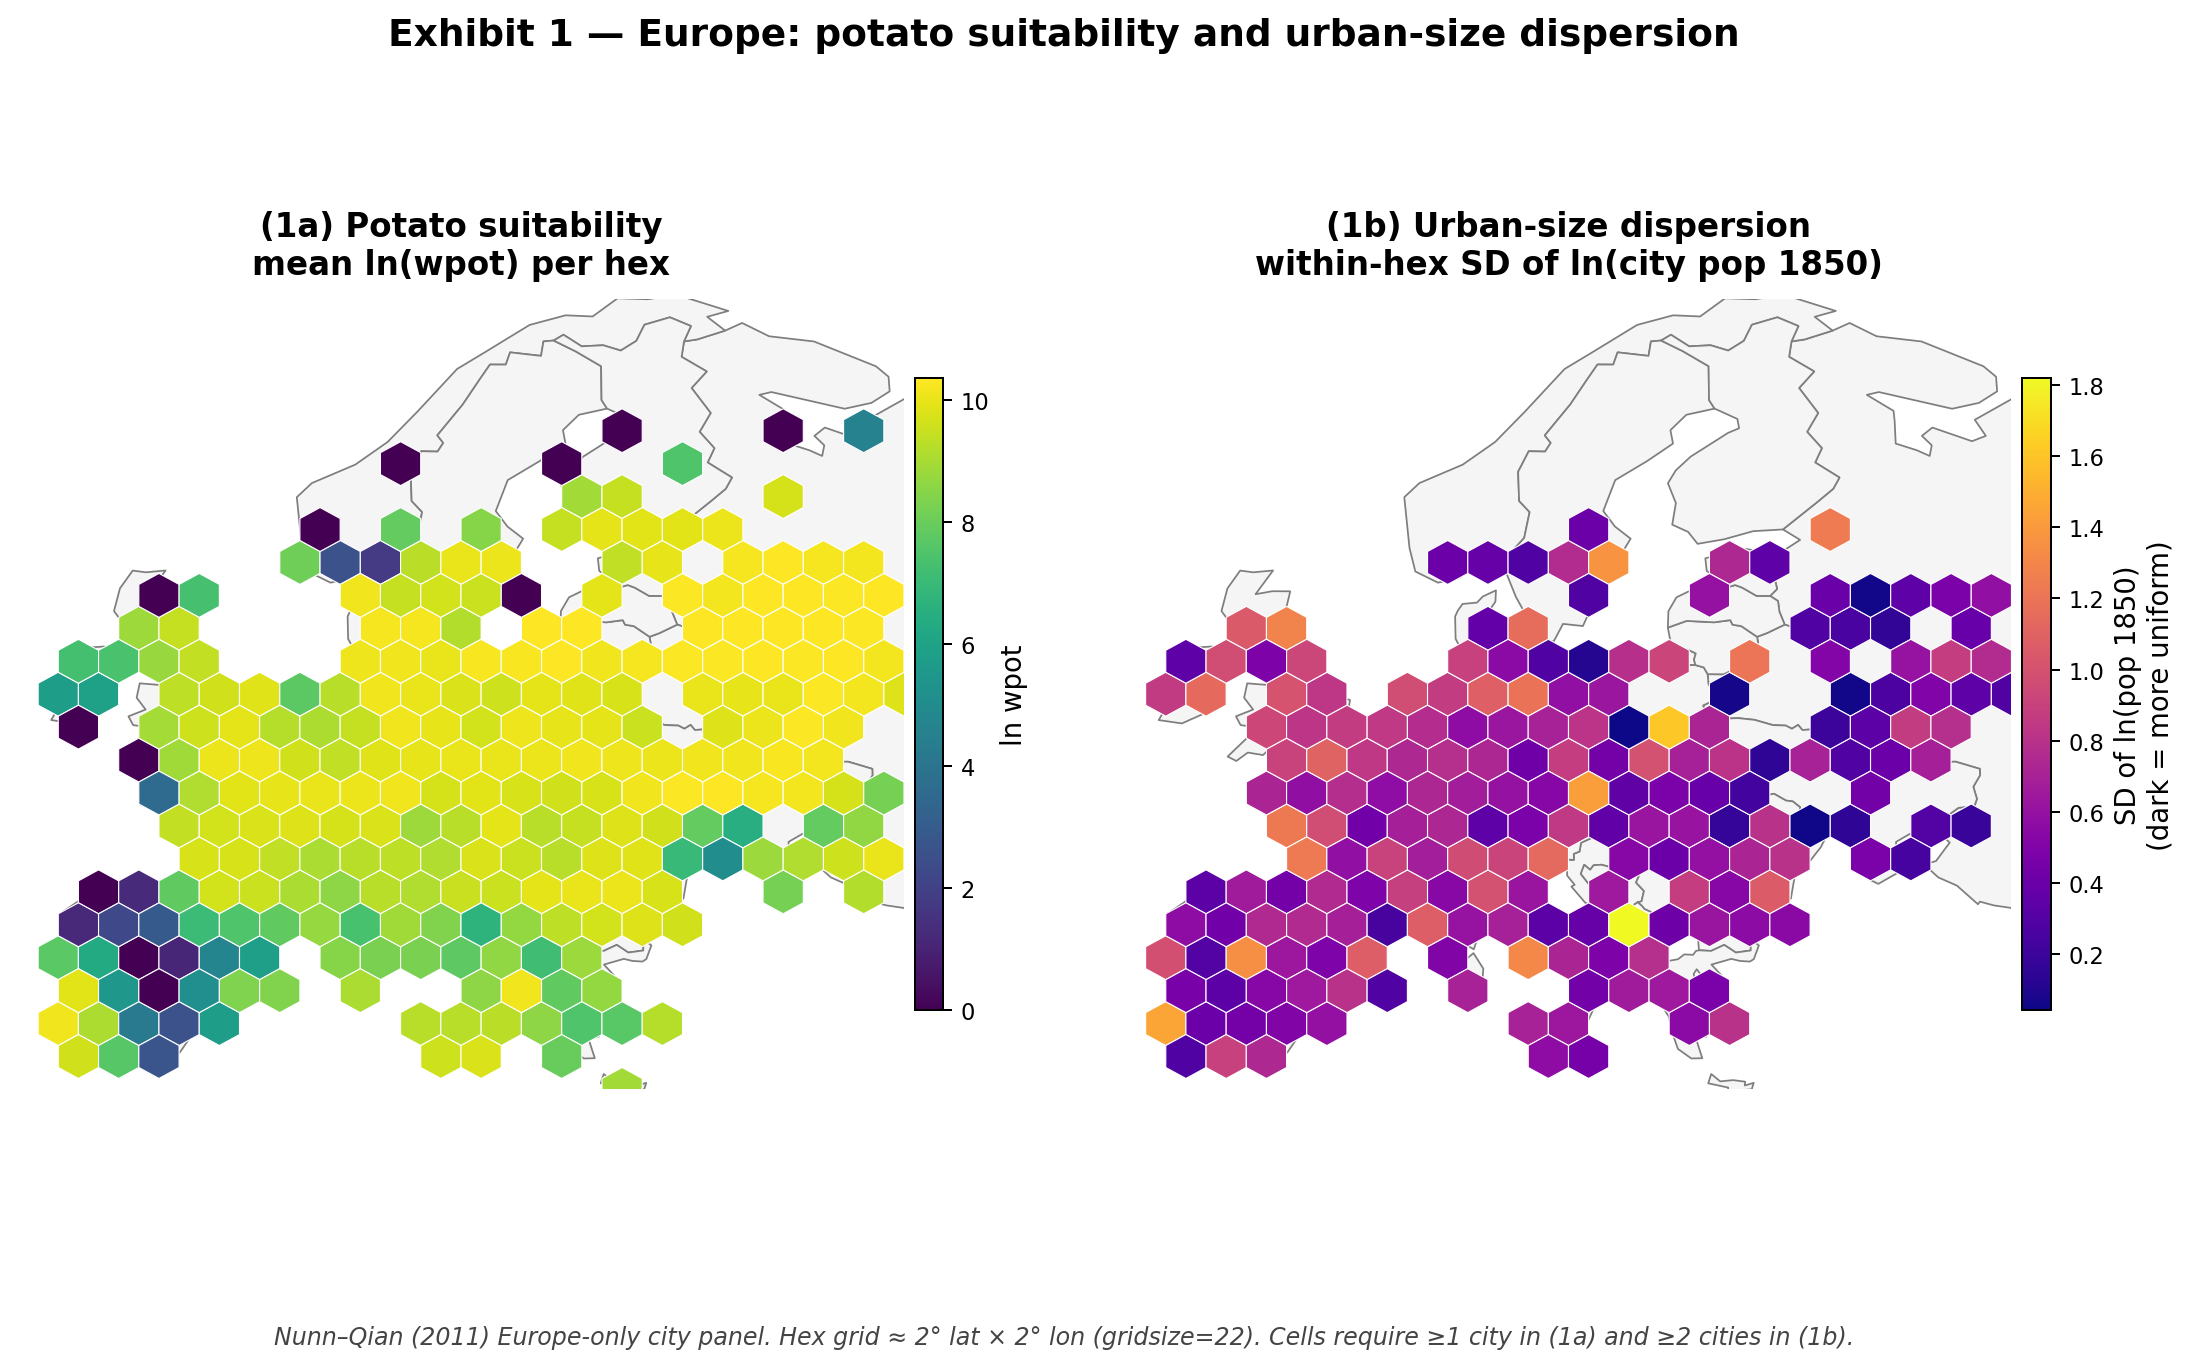
\includegraphics[width=0.95\linewidth]{exhibit1_europe.png}
\caption[Europe: potato suitability and urban-size dispersion]%
{\textbf{Europe: potato suitability and urban-size dispersion.}
Hex-binned heatmaps of the Nunn--Qian Europe-only city panel
($N = 2{,}168$ cities in the plotted bounding box).  Panel (1a)
colors each hex by the mean of $\ln \texttt{wpot}$ across cities in
the cell; brighter cells indicate higher potato suitability. Panel
(1b) colors each hex by the within-hex SD of $\ln$(city pop 1850),
a visual analogue of within-region urban-size dispersion; darker
cells indicate \emph{lower} dispersion (a more uniform urban
hierarchy). Hex grid $\approx 2^{\circ}$ lat $\times\, 2^{\circ}$
lon. Cells require at least one city in (1a) and at least two in
(1b).}
\label{fig:europe_exhibit}
\end{figure}

% =============================================================
%  FIGURE 2.  France: potato suitability vs height dispersion.
% =============================================================

\begin{figure}[!htbp]\centering
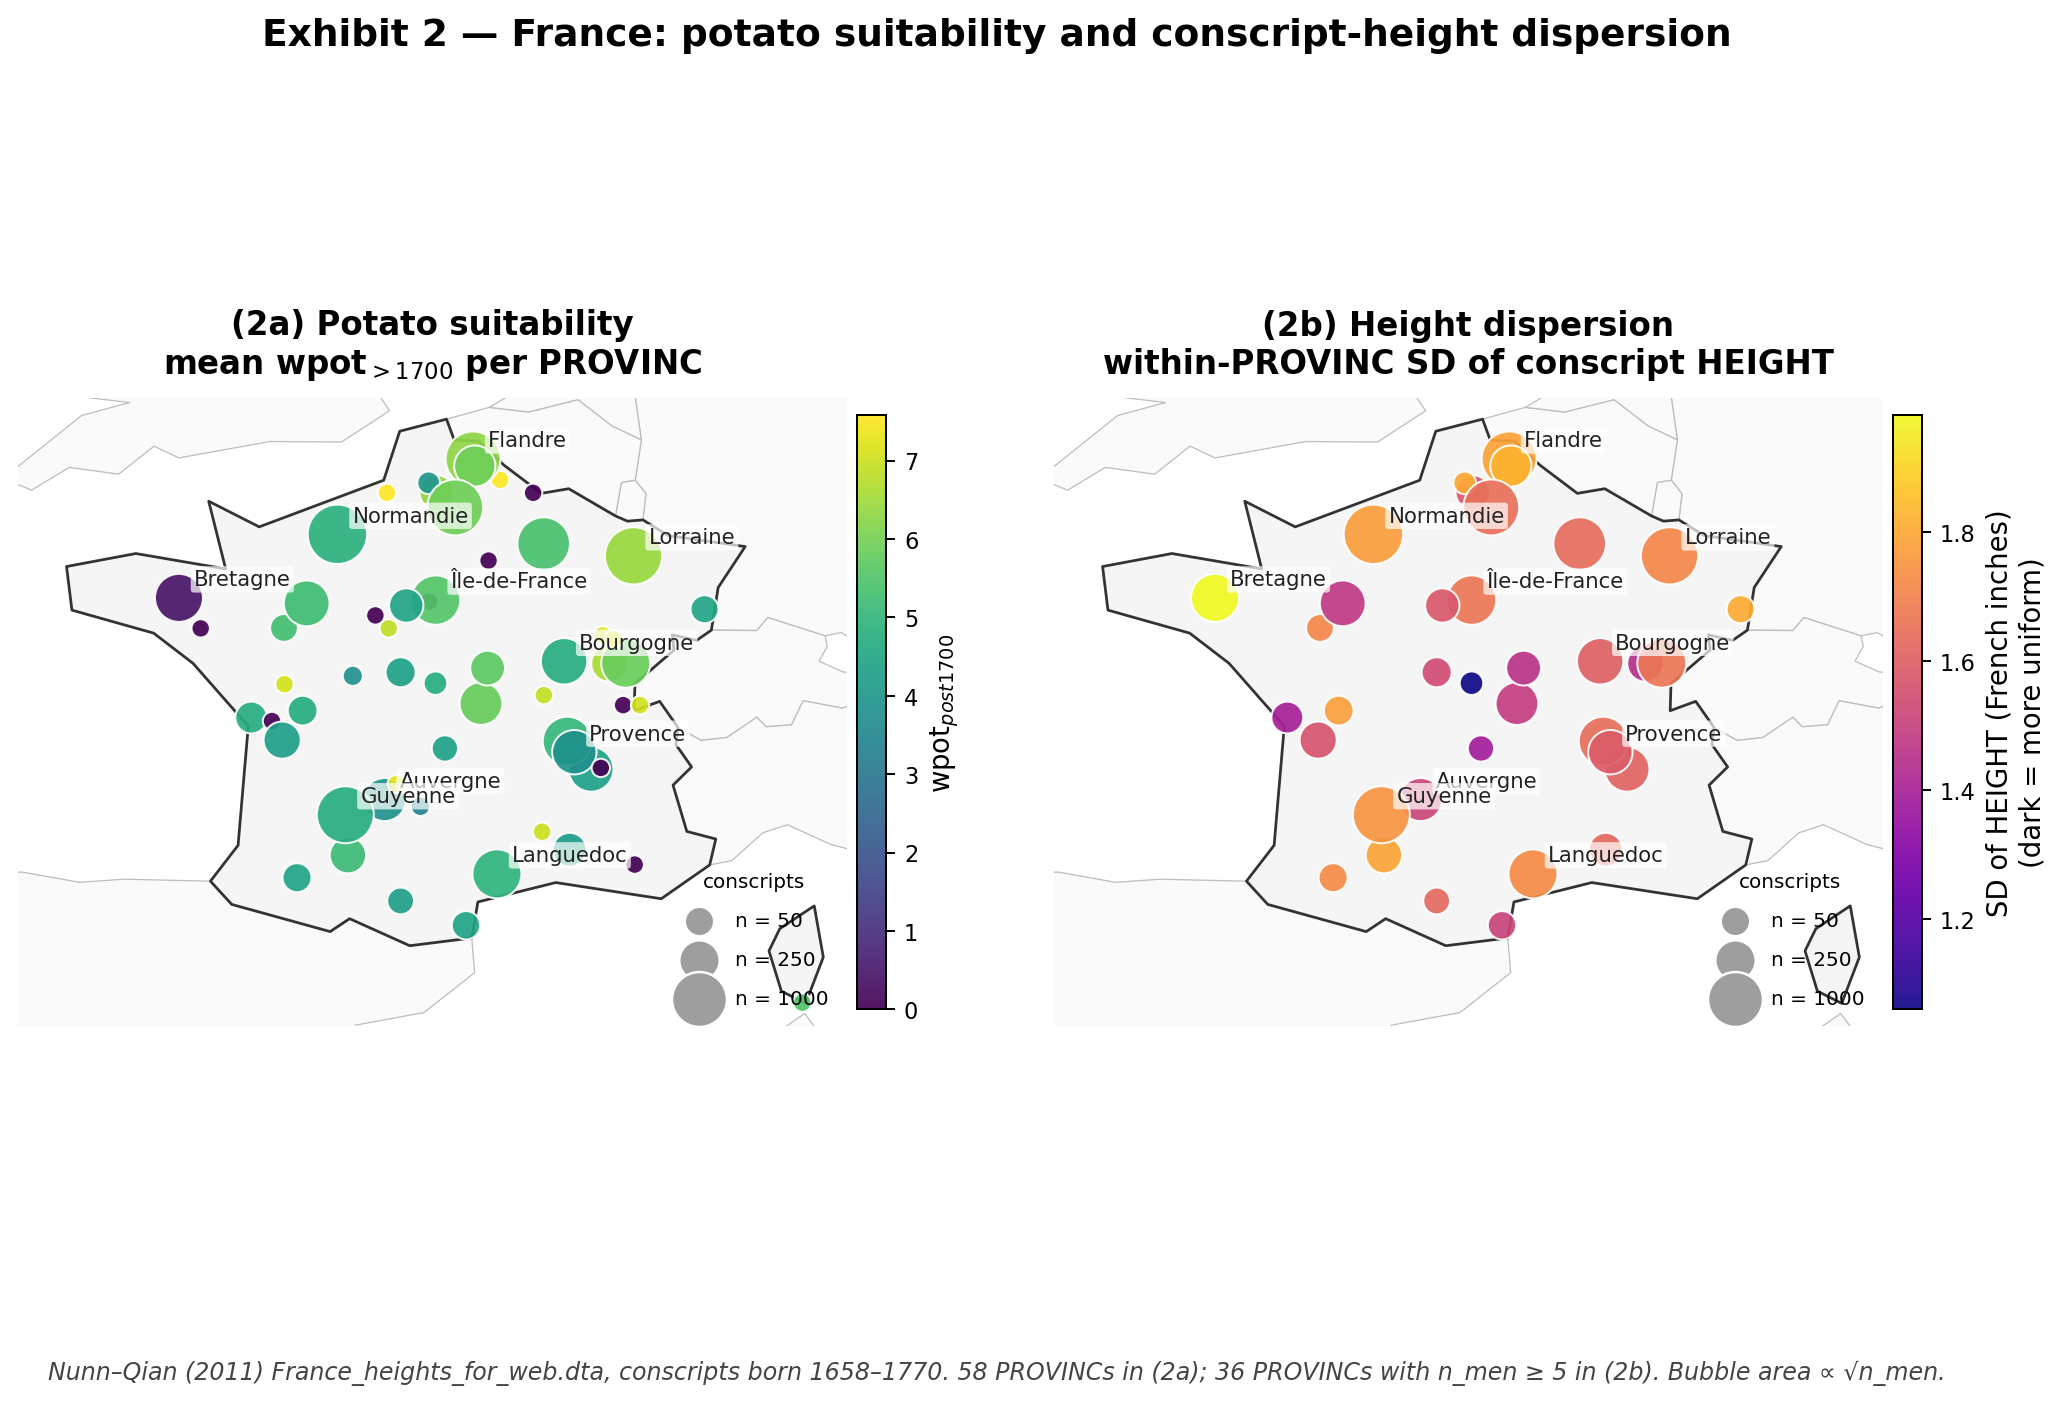
\includegraphics[width=0.95\linewidth]{exhibit2_france.png}
\caption[France: potato suitability and conscript-height dispersion]%
{\textbf{France: potato suitability and conscript-height
dispersion.}  Each département (PROVINC) is plotted at its
conscript-weighted centroid; bubble area is proportional to
$\sqrt{n_{\text{men}}}$. Panel (2a) colors bubbles by the
département mean of \texttt{wpot\_post1700}, the Nunn--Qian post-1700
potato suitability index; brighter bubbles indicate higher
suitability. Panel (2b) restricts to départements with at least
five conscripts ($N = 36$) and colors bubbles by the within-département
SD of conscript HEIGHT (in French inches); darker bubbles indicate
\emph{lower} dispersion (a more uniform local distribution of
physical welfare). Selected major départements are labeled in both
panels.}
\label{fig:france_exhibit}
\end{figure}

% =============================================================
%  FIGURE 3.  Headline regression binscatter.
% =============================================================

\begin{figure}[!htbp]\centering
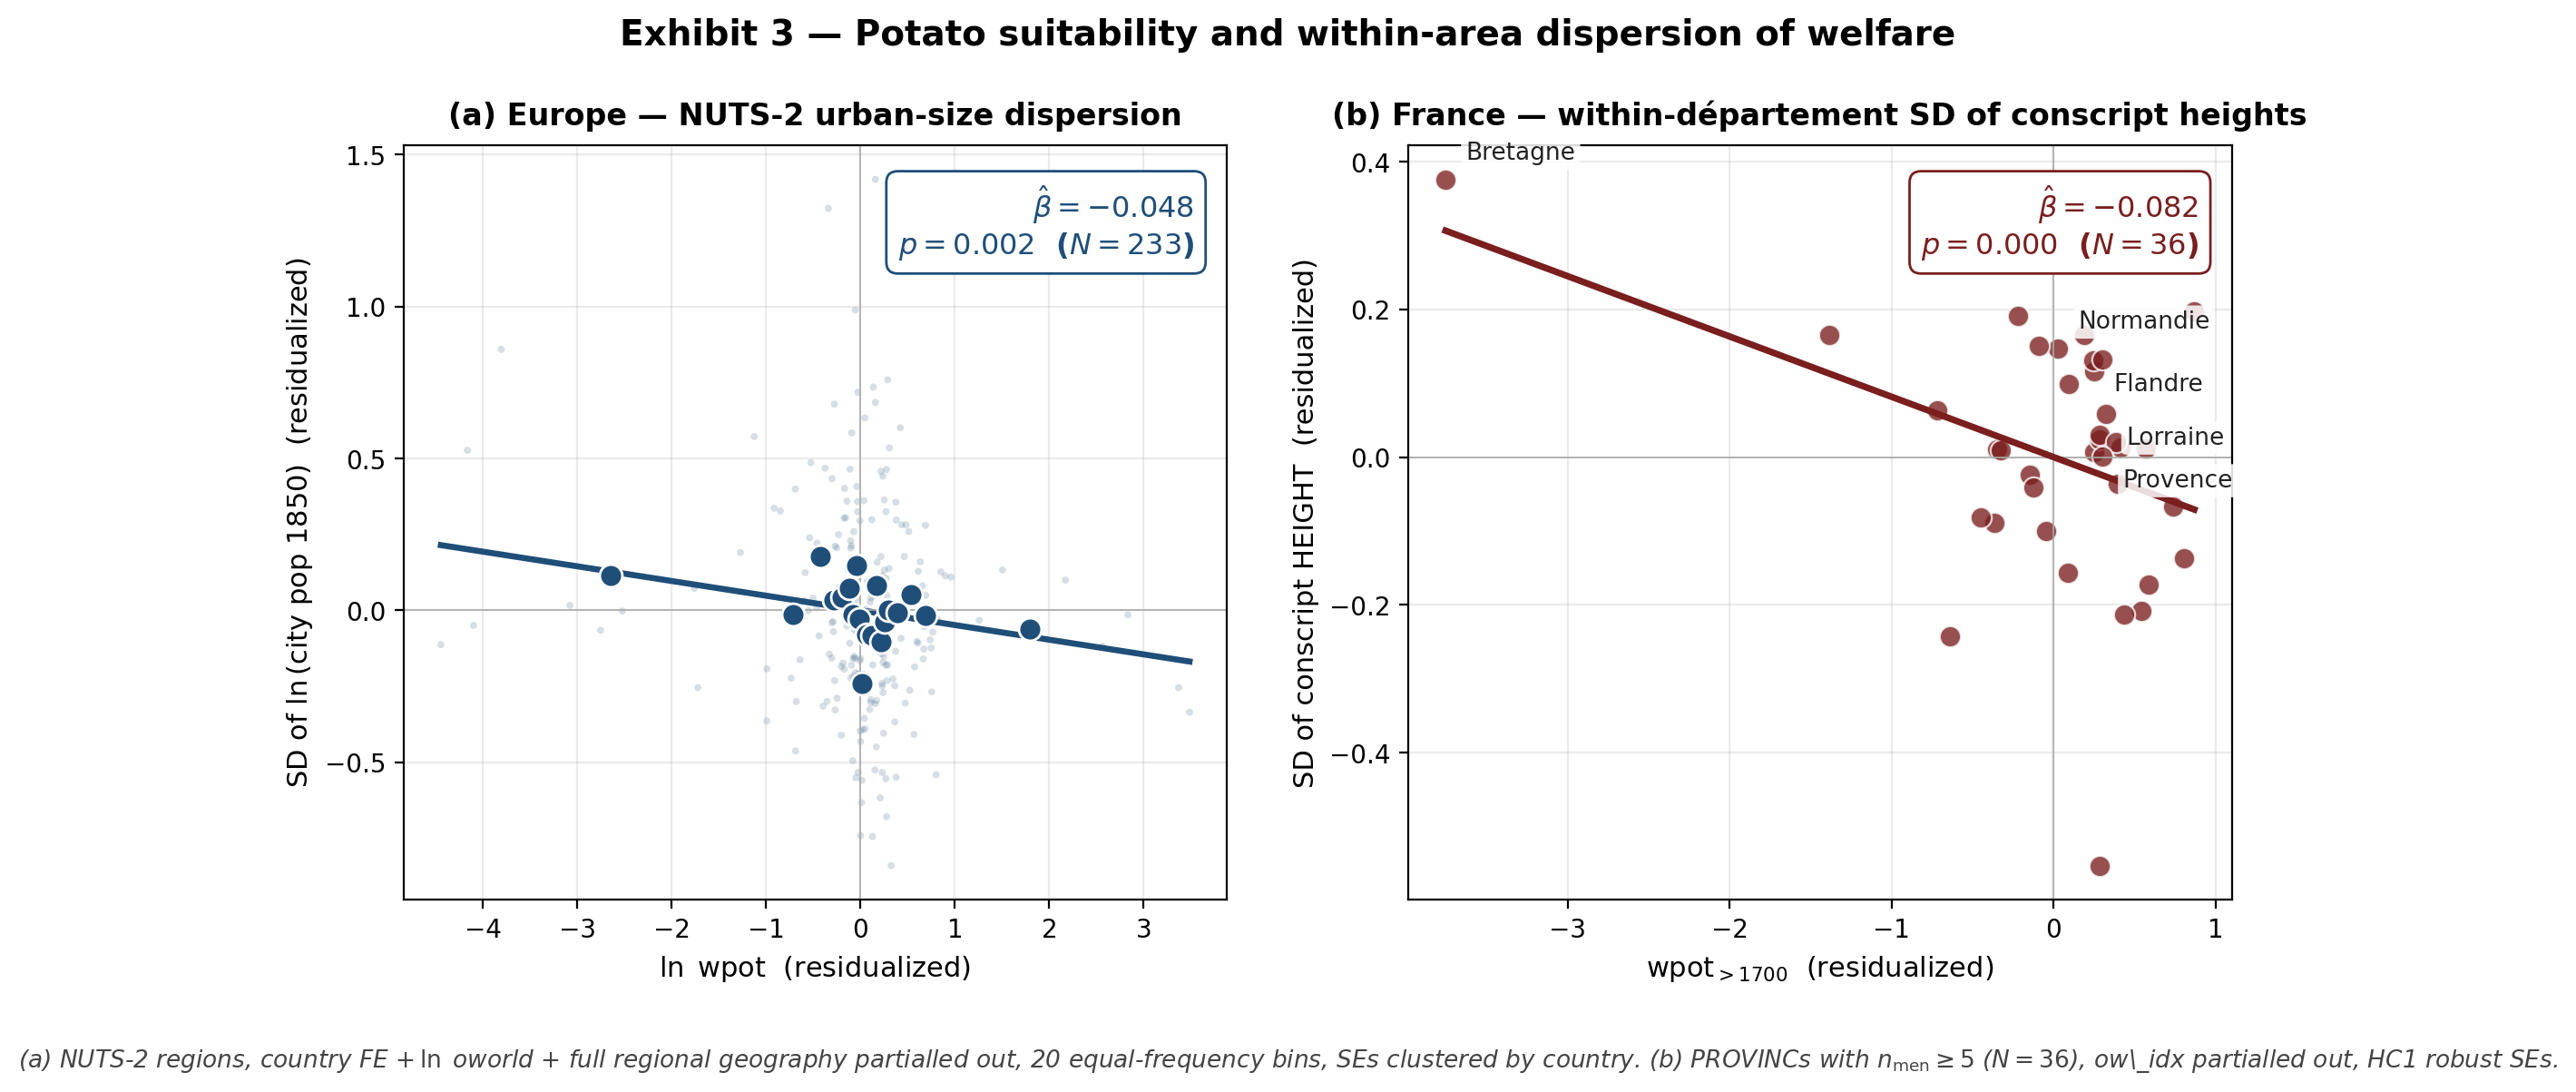
\includegraphics[width=0.95\linewidth]{exhibit3_binscatter.png}
\caption[Potato suitability and within-area dispersion of welfare ---
         partial-regression binscatter]%
{\textbf{Potato suitability and within-area dispersion of welfare:
partial-regression binscatter.} Panel (a) plots residualized
within-region SD of $\ln$(city pop 1850) against residualized
$\ln \texttt{wpot}$ at the NUTS-2 level, after partialling out
country fixed effects, $\ln \texttt{oworld}$, and the remaining
pre-treatment ecological controls ($\ln \texttt{elevation}$,
$\ln \texttt{tropics}$, $\ln \texttt{rugged}$). Twenty
equal-frequency bin means (filled markers) are overlaid on the
underlying residuals (faint markers) together with the OLS fit;
the slope corresponds to the reported regression coefficient. Panel
(b) plots residualized within-département SD of conscript HEIGHT
against residualized $\texttt{wpot\_post1700}$ at the PROVINC level
($N = 36$), with the département-mean of the old-world-suitability
index (\texttt{ow\_idx}) partialled out. Selected outlier
départements are labeled. Standard errors are clustered by country
in (a) and HC1 robust in (b).}
\label{fig:binscatter}
\end{figure}
